\documentclass{book}
\usepackage[landscape,a3paper,left=0.5cm,right=1in,top=1in,bottom=1in]{geometry}
\usepackage{amsmath}
\usepackage{xcolor}
\usepackage{tikz}
\usepackage{pgfplots}
\usepackage{booktabs}
\usepackage{multirow}
\usepackage{amsmath,amssymb}

\begin{document}

\vspace{2cm}

\begin{center}\underline{\textsc{Equiv + Permut} for Test of 98 small instances of polynomial}
\vspace{0.5cm}

\begin{tabular}{ccc} & cp-sat & chuffed\\\\\tikz{\node (a) at (0.0,4) {\textsc{QuadraMod}};\node (a) at (0.0,0) {};} & 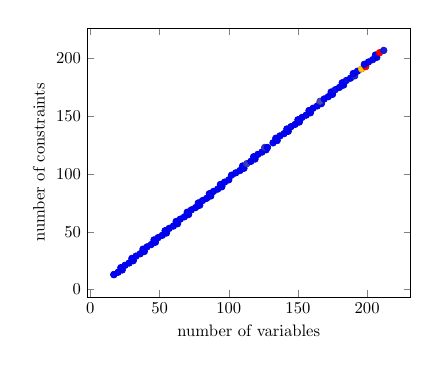
\begin{tikzpicture}[scale=0.6]
\begin{axis}[scatter, point meta=\thisrow{time}, only marks, colorbar, colorbar horizontal,colorbar style={ylabel={Time (min)}, ylabel style={rotate=270},}, colorbar to name={storedcolorbar1},, xlabel=number of variables,ylabel=number of constraints]

\addplot table[x=x,y=y]  { 
 x y time
 17 13 0.05 
 17 13 0.0 
 20 15 0.0 
 23 17 0.0 
 22 19 0.0 
 25 21 0.0 
 28 23 0.0 
 31 25 0.0 
 30 27 0.0 
 33 29 0.0 
 36 31 0.0 
 39 33 0.0 
 38 35 0.0 
 41 37 0.0 
 44 39 0.0 
 47 41 0.0 
 46 43 0.0 
 49 45 0.0 
 52 47 0.0 
 55 49 0.0 
 54 51 0.0 
 57 53 0.0 
 60 55 0.0 
 63 57 0.0 
 62 59 0.0 
 65 61 0.0 
 68 63 0.0 
 71 65 0.0 
 70 67 0.0 
 73 69 0.0 
 76 71 0.0 
 79 73 0.0 
 78 75 0.0 
 81 77 0.0 
 84 79 2.0 
 87 81 0.0 
 86 83 0.0 
 89 85 0.0 
 92 87 0.0 
 95 89 0.0 
 94 91 0.0 
 97 93 1.0 
 100 95 0.0 
 102 99 0.0 
 105 101 3.0 
 108 103 1.0 
 111 105 1.0 
 110 107 1.0 
 113 109 108.0 
 116 111 1.0 
 119 113 1.0 
 118 115 1.0 
 121 117 1.0 
 124 119 1.0 
 127 121 2.0 
 126 123 94.0 
 128 123 1.0 
 132 127 2.0 
 135 129 1.0 
 134 131 2.0 
 137 133 1.0 
 140 135 1.0 
 143 137 2.0 
 142 139 2.0 
 145 141 2.0 
 148 143 2.0 
 151 145 2.0 
 150 147 3.0 
 153 149 3.0 
 156 151 3.0 
 159 153 3.0 
 158 155 3.0 
 161 157 4.0 
 164 159 3.0 
 167 161 4.0 
 166 163 140.0 
 169 165 4.0 
 172 167 4.0 
 175 169 4.0 
 174 171 4.0 
 177 173 21.0 
 180 175 5.0 
 183 177 7.0 
 182 179 5.0 
 185 181 19.0 
 188 183 8.0 
 191 185 59.0 
 190 187 4.0 
 193 189 6.0 
 196 191 678.0 
 199 193 1440.0 
 198 195 7.0 
 201 197 7.0 
 204 199 8.0 
 207 201 8.0 
 206 203 9.0 
 209 205 1440.0 
 212 207 47.0 
};

\end{axis}
\end{tikzpicture}

 & 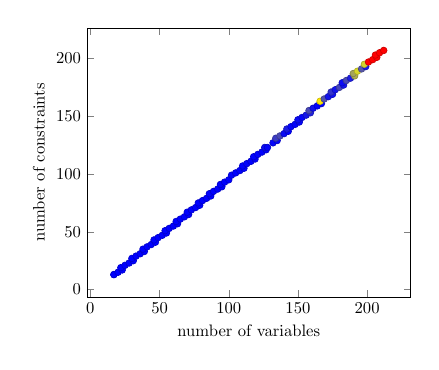
\begin{tikzpicture}[scale=0.6]
\begin{axis}[scatter, point meta=\thisrow{time}, only marks, , xlabel=number of variables,ylabel=number of constraints]

\addplot table[x=x,y=y]  { 
 x y time
 17 13 0.05 
 17 13 0.0 
 20 15 0.0 
 23 17 0.0 
 22 19 0.0 
 25 21 0.0 
 28 23 0.0 
 31 25 0.0 
 30 27 0.0 
 33 29 0.0 
 36 31 0.0 
 39 33 0.0 
 38 35 0.0 
 41 37 0.0 
 44 39 0.0 
 47 41 0.0 
 46 43 0.0 
 49 45 0.0 
 52 47 0.0 
 55 49 0.0 
 54 51 0.0 
 57 53 1.0 
 60 55 0.0 
 63 57 1.0 
 62 59 0.0 
 65 61 0.0 
 68 63 0.0 
 71 65 2.0 
 70 67 0.0 
 73 69 2.0 
 76 71 0.0 
 79 73 1.0 
 78 75 1.0 
 81 77 1.0 
 84 79 1.0 
 87 81 1.0 
 86 83 4.0 
 89 85 2.0 
 92 87 2.0 
 95 89 2.0 
 94 91 2.0 
 97 93 2.0 
 100 95 2.0 
 102 99 5.0 
 105 101 2.0 
 108 103 4.0 
 111 105 2.0 
 110 107 3.0 
 113 109 5.0 
 116 111 2.0 
 119 113 2.0 
 118 115 3.0 
 121 117 3.0 
 124 119 3.0 
 127 121 4.0 
 126 123 23.0 
 128 123 10.0 
 132 127 12.0 
 135 129 9.0 
 134 131 110.0 
 137 133 138.0 
 140 135 22.0 
 143 137 6.0 
 142 139 50.0 
 145 141 7.0 
 148 143 7.0 
 151 145 12.0 
 150 147 21.0 
 153 149 11.0 
 156 151 41.0 
 159 153 62.0 
 158 155 137.0 
 161 157 34.0 
 164 159 8.0 
 167 161 14.0 
 166 163 568.0 
 169 165 157.0 
 172 167 37.0 
 175 169 26.0 
 174 171 92.0 
 177 173 36.0 
 180 175 130.0 
 183 177 37.0 
 182 179 22.0 
 185 181 136.0 
 188 183 57.0 
 191 185 329.0 
 190 187 309.0 
 193 189 404.0 
 196 191 164.0 
 199 193 44.0 
 198 195 394.0 
 201 197 1440.0 
 204 199 1440.0 
 207 201 1440.0 
 206 203 1440.0 
 209 205 1440.0 
 212 207 1440.0 
};

\end{axis}
\end{tikzpicture}

\\
\tikz{\node (a) at (0.0,4) {\textsc{TheoMod}};\node (a) at (0.0,0) {};} & 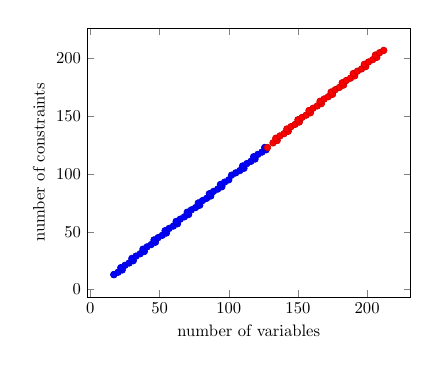
\begin{tikzpicture}[scale=0.6]
\begin{axis}[scatter, point meta=\thisrow{time}, only marks, , xlabel=number of variables,ylabel=number of constraints]

\addplot table[x=x,y=y]  { 
 x y time
 17 13 0.05 
 17 13 0.0 
 20 15 0.0 
 23 17 0.0 
 22 19 0.0 
 25 21 0.0 
 28 23 0.0 
 31 25 0.0 
 30 27 0.0 
 33 29 0.0 
 36 31 0.0 
 39 33 0.0 
 38 35 0.0 
 41 37 0.0 
 44 39 0.0 
 47 41 0.0 
 46 43 0.0 
 49 45 0.0 
 52 47 0.0 
 55 49 0.0 
 54 51 0.0 
 57 53 0.0 
 60 55 0.0 
 63 57 0.0 
 62 59 0.0 
 65 61 0.0 
 68 63 0.0 
 71 65 0.0 
 70 67 0.0 
 73 69 0.0 
 76 71 0.0 
 79 73 0.0 
 78 75 0.0 
 81 77 1.0 
 84 79 0.0 
 87 81 1.0 
 86 83 1.0 
 89 85 1.0 
 92 87 1.0 
 95 89 1.0 
 94 91 1.0 
 97 93 2.0 
 100 95 1.0 
 102 99 2.0 
 105 101 2.0 
 108 103 2.0 
 111 105 3.0 
 110 107 2.0 
 113 109 3.0 
 116 111 3.0 
 119 113 3.0 
 118 115 3.0 
 121 117 4.0 
 124 119 4.0 
 127 121 5.0 
 126 123 5.0 
 128 123 1440.0 
 132 127 1440.0 
 135 129 1440.0 
 134 131 1440.0 
 137 133 1440.0 
 140 135 1440.0 
 143 137 1440.0 
 142 139 1440.0 
 145 141 1440.0 
 148 143 1440.0 
 151 145 1440.0 
 150 147 1440.0 
 153 149 1440.0 
 156 151 1440.0 
 159 153 1440.0 
 158 155 1440.0 
 161 157 1440.0 
 164 159 1440.0 
 167 161 1440.0 
 166 163 1440.0 
 169 165 1440.0 
 172 167 1440.0 
 175 169 1440.0 
 174 171 1440.0 
 177 173 1440.0 
 180 175 1440.0 
 183 177 1440.0 
 182 179 1440.0 
 185 181 1440.0 
 188 183 1440.0 
 191 185 1440.0 
 190 187 1440.0 
 193 189 1440.0 
 196 191 1440.0 
 199 193 1440.0 
 198 195 1440.0 
 201 197 1440.0 
 204 199 1440.0 
 207 201 1440.0 
 206 203 1440.0 
 209 205 1440.0 
 212 207 1440.0 
};

\end{axis}
\end{tikzpicture}

 & 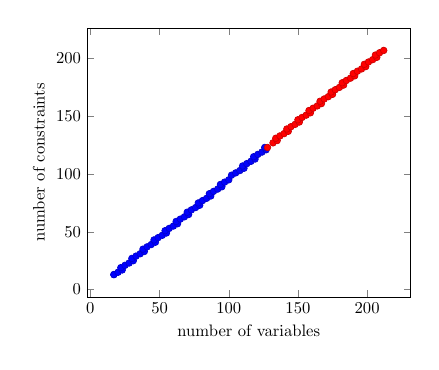
\begin{tikzpicture}[scale=0.6]
\begin{axis}[scatter, point meta=\thisrow{time}, only marks, , xlabel=number of variables,ylabel=number of constraints]

\addplot table[x=x,y=y]  { 
 x y time
 17 13 0.05 
 17 13 0.0 
 20 15 0.0 
 23 17 0.0 
 22 19 0.0 
 25 21 0.0 
 28 23 0.0 
 31 25 0.0 
 30 27 0.0 
 33 29 0.0 
 36 31 0.0 
 39 33 0.0 
 38 35 0.0 
 41 37 0.0 
 44 39 0.0 
 47 41 0.0 
 46 43 0.0 
 49 45 0.0 
 52 47 0.0 
 55 49 0.0 
 54 51 0.0 
 57 53 0.0 
 60 55 0.0 
 63 57 1.0 
 62 59 0.0 
 65 61 0.0 
 68 63 0.0 
 71 65 1.0 
 70 67 2.0 
 73 69 3.0 
 76 71 4.0 
 79 73 1.0 
 78 75 1.0 
 81 77 1.0 
 84 79 2.0 
 87 81 2.0 
 86 83 2.0 
 89 85 5.0 
 92 87 4.0 
 95 89 4.0 
 94 91 4.0 
 97 93 3.0 
 100 95 5.0 
 102 99 6.0 
 105 101 7.0 
 108 103 13.0 
 111 105 7.0 
 110 107 12.0 
 113 109 7.0 
 116 111 8.0 
 119 113 9.0 
 118 115 9.0 
 121 117 10.0 
 124 119 11.0 
 127 121 12.0 
 126 123 11.0 
 128 123 1440.0 
 132 127 1440.0 
 135 129 1440.0 
 134 131 1440.0 
 137 133 1440.0 
 140 135 1440.0 
 143 137 1440.0 
 142 139 1440.0 
 145 141 1440.0 
 148 143 1440.0 
 151 145 1440.0 
 150 147 1440.0 
 153 149 1440.0 
 156 151 1440.0 
 159 153 1440.0 
 158 155 1440.0 
 161 157 1440.0 
 164 159 1440.0 
 167 161 1440.0 
 166 163 1440.0 
 169 165 1440.0 
 172 167 1440.0 
 175 169 1440.0 
 174 171 1440.0 
 177 173 1440.0 
 180 175 1440.0 
 183 177 1440.0 
 182 179 1440.0 
 185 181 1440.0 
 188 183 1440.0 
 191 185 1440.0 
 190 187 1440.0 
 193 189 1440.0 
 196 191 1440.0 
 199 193 1440.0 
 198 195 1440.0 
 201 197 1440.0 
 204 199 1440.0 
 207 201 1440.0 
 206 203 1440.0 
 209 205 1440.0 
 212 207 1440.0 
};

\end{axis}
\end{tikzpicture}

\\
\\\\
\multicolumn{3}{c}{\ref{storedcolorbar1}}\end{tabular}\end{center}

\newpage

\begin{center}\underline{\textsc{Non-Equiv + Permut} for Test of 98 small instances of polynomial}
\vspace{0.5cm}

\begin{tabular}{ccc} & cp-sat & chuffed\\\\\tikz{\node (a) at (0.0,4) {\textsc{QuadraMod}};\node (a) at (0.0,0) {};} & 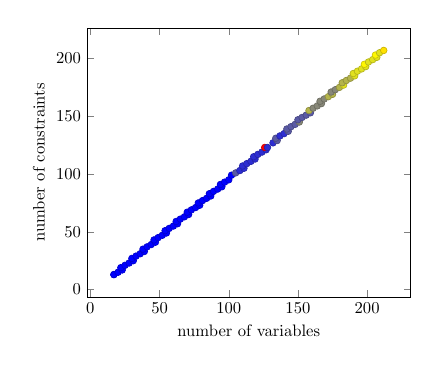
\begin{tikzpicture}[scale=0.6]
\begin{axis}[scatter, point meta=\thisrow{time}, only marks, colorbar, colorbar horizontal,colorbar style={ylabel={Time (min)}, ylabel style={rotate=270},}, colorbar to name={storedcolorbar2},, xlabel=number of variables,ylabel=number of constraints]

\addplot table[x=x,y=y]  { 
 x y time
 17 13 0.05 
 17 13 0.0 
 20 15 0.0 
 23 17 0.0 
 22 19 0.0 
 25 21 0.0 
 28 23 0.0 
 31 25 0.0 
 30 27 0.0 
 33 29 0.0 
 36 31 0.0 
 39 33 0.0 
 38 35 0.0 
 41 37 0.0 
 44 39 0.0 
 47 41 0.0 
 46 43 0.0 
 49 45 0.0 
 52 47 0.0 
 55 49 0.0 
 54 51 0.0 
 57 53 0.0 
 60 55 0.0 
 63 57 0.0 
 62 59 0.0 
 65 61 0.0 
 68 63 0.0 
 71 65 0.0 
 70 67 0.0 
 73 69 0.0 
 76 71 0.0 
 79 73 0.0 
 78 75 0.0 
 81 77 0.0 
 84 79 0.0 
 87 81 0.0 
 86 83 0.0 
 89 85 0.0 
 92 87 0.0 
 95 89 0.0 
 94 91 0.0 
 97 93 0.0 
 100 95 0.0 
 102 99 0.0 
 105 101 2.0 
 108 103 1.0 
 111 105 1.0 
 110 107 1.0 
 113 109 1.0 
 116 111 1.0 
 119 113 1.0 
 118 115 1.0 
 121 117 1.0 
 124 119 1.0 
 127 121 1.0 
 126 123 17.0 
 128 123 1.0 
 132 127 1.0 
 135 129 2.0 
 134 131 2.0 
 137 133 1.0 
 140 135 1.0 
 143 137 2.0 
 142 139 2.0 
 145 141 2.0 
 148 143 2.0 
 151 145 3.0 
 150 147 2.0 
 153 149 2.0 
 156 151 2.0 
 159 153 2.0 
 158 155 4.0 
 161 157 3.0 
 164 159 3.0 
 167 161 3.0 
 166 163 3.0 
 169 165 3.0 
 172 167 4.0 
 175 169 4.0 
 174 171 3.0 
 177 173 3.0 
 180 175 4.0 
 183 177 5.0 
 182 179 4.0 
 185 181 4.0 
 188 183 4.0 
 191 185 5.0 
 190 187 5.0 
 193 189 5.0 
 196 191 5.0 
 199 193 5.0 
 198 195 6.0 
 201 197 5.0 
 204 199 5.0 
 207 201 5.0 
 206 203 6.0 
 209 205 5.0 
 212 207 7.0 
};

\end{axis}
\end{tikzpicture}

 & 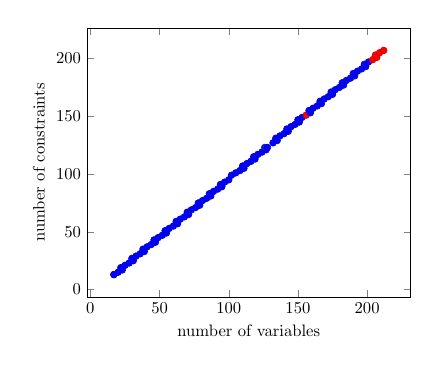
\begin{tikzpicture}[scale=0.6]
\begin{axis}[scatter, point meta=\thisrow{time}, only marks, , xlabel=number of variables,ylabel=number of constraints]

\addplot table[x=x,y=y]  { 
 x y time
 17 13 0.05 
 17 13 0.0 
 20 15 0.0 
 23 17 0.0 
 22 19 0.0 
 25 21 0.0 
 28 23 0.0 
 31 25 0.0 
 30 27 0.0 
 33 29 0.0 
 36 31 0.0 
 39 33 0.0 
 38 35 0.0 
 41 37 0.0 
 44 39 0.0 
 47 41 0.0 
 46 43 0.0 
 49 45 0.0 
 52 47 0.0 
 55 49 0.0 
 54 51 0.0 
 57 53 0.0 
 60 55 0.0 
 63 57 0.0 
 62 59 0.0 
 65 61 1.0 
 68 63 1.0 
 71 65 0.0 
 70 67 1.0 
 73 69 0.0 
 76 71 1.0 
 79 73 1.0 
 78 75 0.0 
 81 77 1.0 
 84 79 2.0 
 87 81 1.0 
 86 83 1.0 
 89 85 2.0 
 92 87 2.0 
 95 89 2.0 
 94 91 4.0 
 97 93 3.0 
 100 95 2.0 
 102 99 2.0 
 105 101 3.0 
 108 103 2.0 
 111 105 3.0 
 110 107 3.0 
 113 109 4.0 
 116 111 2.0 
 119 113 2.0 
 118 115 3.0 
 121 117 3.0 
 124 119 3.0 
 127 121 4.0 
 126 123 45.0 
 128 123 3.0 
 132 127 4.0 
 135 129 4.0 
 134 131 4.0 
 137 133 4.0 
 140 135 5.0 
 143 137 6.0 
 142 139 4.0 
 145 141 5.0 
 148 143 5.0 
 151 145 5.0 
 150 147 6.0 
 153 149 6.0 
 156 151 1440.0 
 159 153 8.0 
 158 155 7.0 
 161 157 8.0 
 164 159 8.0 
 167 161 7.0 
 166 163 7.0 
 169 165 8.0 
 172 167 9.0 
 175 169 9.0 
 174 171 10.0 
 177 173 10.0 
 180 175 10.0 
 183 177 10.0 
 182 179 11.0 
 185 181 12.0 
 188 183 12.0 
 191 185 13.0 
 190 187 13.0 
 193 189 13.0 
 196 191 14.0 
 199 193 14.0 
 198 195 14.0 
 201 197 14.0 
 204 199 1440.0 
 207 201 1440.0 
 206 203 1440.0 
 209 205 1440.0 
 212 207 1440.0 
};

\end{axis}
\end{tikzpicture}

\\
\tikz{\node (a) at (0.0,4) {\textsc{TheoMod}};\node (a) at (0.0,0) {};} & 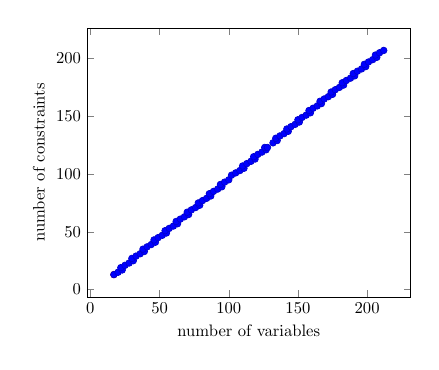
\begin{tikzpicture}[scale=0.6]
\begin{axis}[scatter, point meta=\thisrow{time}, only marks, , xlabel=number of variables,ylabel=number of constraints]

\addplot table[x=x,y=y]  { 
 x y time
 17 13 0.05 
 17 13 0.0 
 20 15 0.0 
 23 17 0.0 
 22 19 0.0 
 25 21 0.0 
 28 23 0.0 
 31 25 0.0 
 30 27 0.0 
 33 29 0.0 
 36 31 0.0 
 39 33 0.0 
 38 35 0.0 
 41 37 0.0 
 44 39 0.0 
 47 41 0.0 
 46 43 0.0 
 49 45 0.0 
 52 47 0.0 
 55 49 0.0 
 54 51 0.0 
 57 53 0.0 
 60 55 0.0 
 63 57 0.0 
 62 59 0.0 
 65 61 0.0 
 68 63 0.0 
 71 65 0.0 
 70 67 0.0 
 73 69 0.0 
 76 71 0.0 
 79 73 0.0 
 78 75 0.0 
 81 77 0.0 
 84 79 0.0 
 87 81 0.0 
 86 83 0.0 
 89 85 0.0 
 92 87 0.0 
 95 89 0.0 
 94 91 0.0 
 97 93 0.0 
 100 95 0.0 
 102 99 0.0 
 105 101 0.0 
 108 103 0.0 
 111 105 0.0 
 110 107 0.0 
 113 109 0.0 
 116 111 0.0 
 119 113 0.0 
 118 115 0.0 
 121 117 0.0 
 124 119 0.0 
 127 121 0.0 
 126 123 0.0 
 128 123 0.0 
 132 127 0.0 
 135 129 0.0 
 134 131 0.0 
 137 133 0.0 
 140 135 0.0 
 143 137 0.0 
 142 139 0.0 
 145 141 0.0 
 148 143 0.0 
 151 145 0.0 
 150 147 0.0 
 153 149 0.0 
 156 151 0.0 
 159 153 0.0 
 158 155 0.0 
 161 157 0.0 
 164 159 0.0 
 167 161 0.0 
 166 163 0.0 
 169 165 0.0 
 172 167 0.0 
 175 169 0.0 
 174 171 0.0 
 177 173 0.0 
 180 175 0.0 
 183 177 0.0 
 182 179 0.0 
 185 181 0.0 
 188 183 0.0 
 191 185 0.0 
 190 187 0.0 
 193 189 0.0 
 196 191 0.0 
 199 193 0.0 
 198 195 0.0 
 201 197 0.0 
 204 199 0.0 
 207 201 0.0 
 206 203 0.0 
 209 205 0.0 
 212 207 0.0 
};

\end{axis}
\end{tikzpicture}

 & 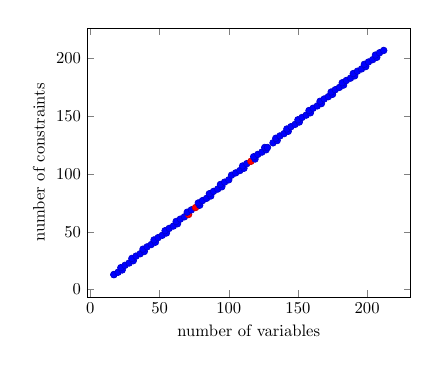
\begin{tikzpicture}[scale=0.6]
\begin{axis}[scatter, point meta=\thisrow{time}, only marks, , xlabel=number of variables,ylabel=number of constraints]

\addplot table[x=x,y=y]  { 
 x y time
 17 13 0.05 
 17 13 0.0 
 20 15 0.0 
 23 17 0.0 
 22 19 0.0 
 25 21 0.0 
 28 23 0.0 
 31 25 0.0 
 30 27 0.0 
 33 29 0.0 
 36 31 0.0 
 39 33 0.0 
 38 35 0.0 
 41 37 0.0 
 44 39 0.0 
 47 41 0.0 
 46 43 0.0 
 49 45 0.0 
 52 47 0.0 
 55 49 0.0 
 54 51 0.0 
 57 53 0.0 
 60 55 0.0 
 63 57 0.0 
 62 59 0.0 
 65 61 0.0 
 68 63 0.0 
 71 65 1440.0 
 70 67 0.0 
 73 69 0.0 
 76 71 1440.0 
 79 73 0.0 
 78 75 0.0 
 81 77 0.0 
 84 79 0.0 
 87 81 0.0 
 86 83 0.0 
 89 85 0.0 
 92 87 0.0 
 95 89 0.0 
 94 91 0.0 
 97 93 0.0 
 100 95 0.0 
 102 99 0.0 
 105 101 0.0 
 108 103 0.0 
 111 105 0.0 
 110 107 0.0 
 113 109 0.0 
 116 111 1440.0 
 119 113 0.0 
 118 115 0.0 
 121 117 0.0 
 124 119 0.0 
 127 121 0.0 
 126 123 2.0 
 128 123 0.0 
 132 127 0.0 
 135 129 0.0 
 134 131 0.0 
 137 133 0.0 
 140 135 0.0 
 143 137 0.0 
 142 139 0.0 
 145 141 0.0 
 148 143 0.0 
 151 145 0.0 
 150 147 0.0 
 153 149 0.0 
 156 151 0.0 
 159 153 0.0 
 158 155 0.0 
 161 157 0.0 
 164 159 0.0 
 167 161 0.0 
 166 163 0.0 
 169 165 0.0 
 172 167 0.0 
 175 169 0.0 
 174 171 0.0 
 177 173 0.0 
 180 175 0.0 
 183 177 0.0 
 182 179 0.0 
 185 181 0.0 
 188 183 0.0 
 191 185 0.0 
 190 187 0.0 
 193 189 0.0 
 196 191 0.0 
 199 193 0.0 
 198 195 0.0 
 201 197 0.0 
 204 199 0.0 
 207 201 0.0 
 206 203 0.0 
 209 205 0.0 
 212 207 0.0 
};

\end{axis}
\end{tikzpicture}

\\
\\\\
\multicolumn{3}{c}{\ref{storedcolorbar2}}\end{tabular}\end{center}

\newpage

\end{document}